\section{Results}\label{sec:results}

\subsection{Experimental Setup}

To study the effect of the mutation rate, we ran the GA with three mutation rates, 0.01, 0.05 and 0.2, each with three random seeds (1, 2 and 3), for a total of 9 runs. All other parameters keep the default values of Table~\ref{tab:params}, so each run evolves a population of 100 melodies of 12 bars for 1250 generations. Each run saves the best melody of generations 0, 311, 624, 936 and 1249 as MIDI and audio files. The code, the audio files and the script that reproduces the experiment are available at \url{https://github.com/Chbmleao/jazz-sax-ga}.

\subsection{Fitness Evolution}

\begin{figure}
  \centering
  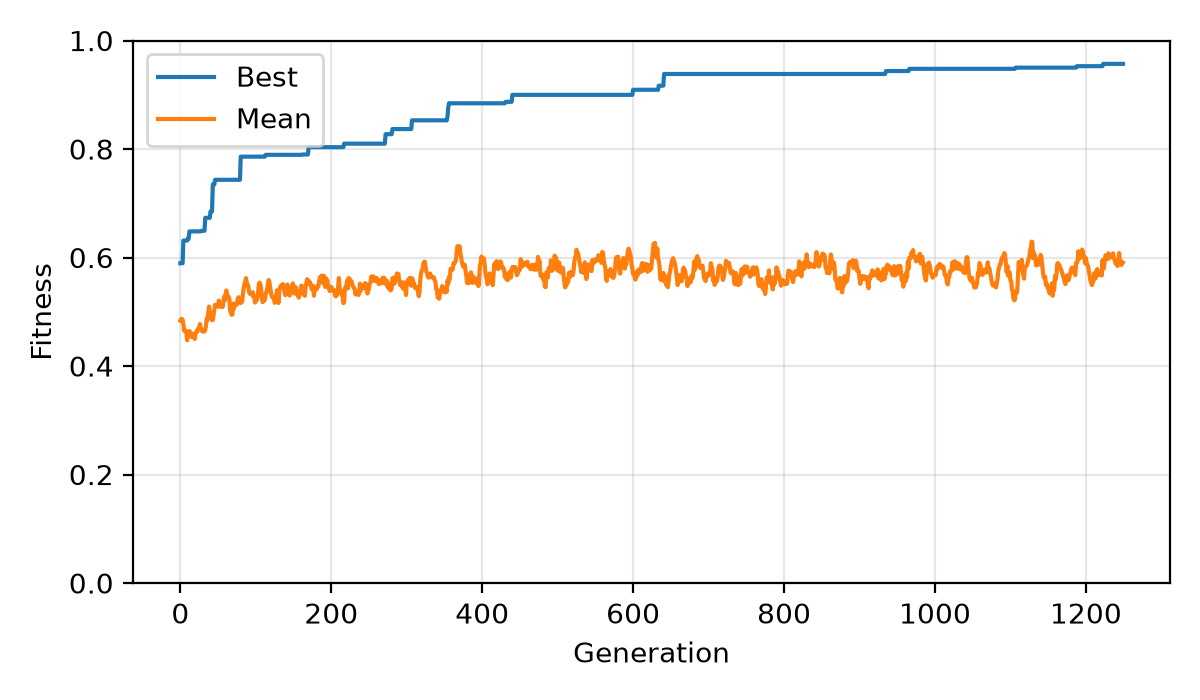
\includegraphics[width=\linewidth]{figures/fitness.png}
  \caption{Best and mean fitness per generation for the default configuration
    (mutation rate 0.01, seed 1).}
  \label{fig:fitness}
\end{figure}

\begin{figure}
  \centering
  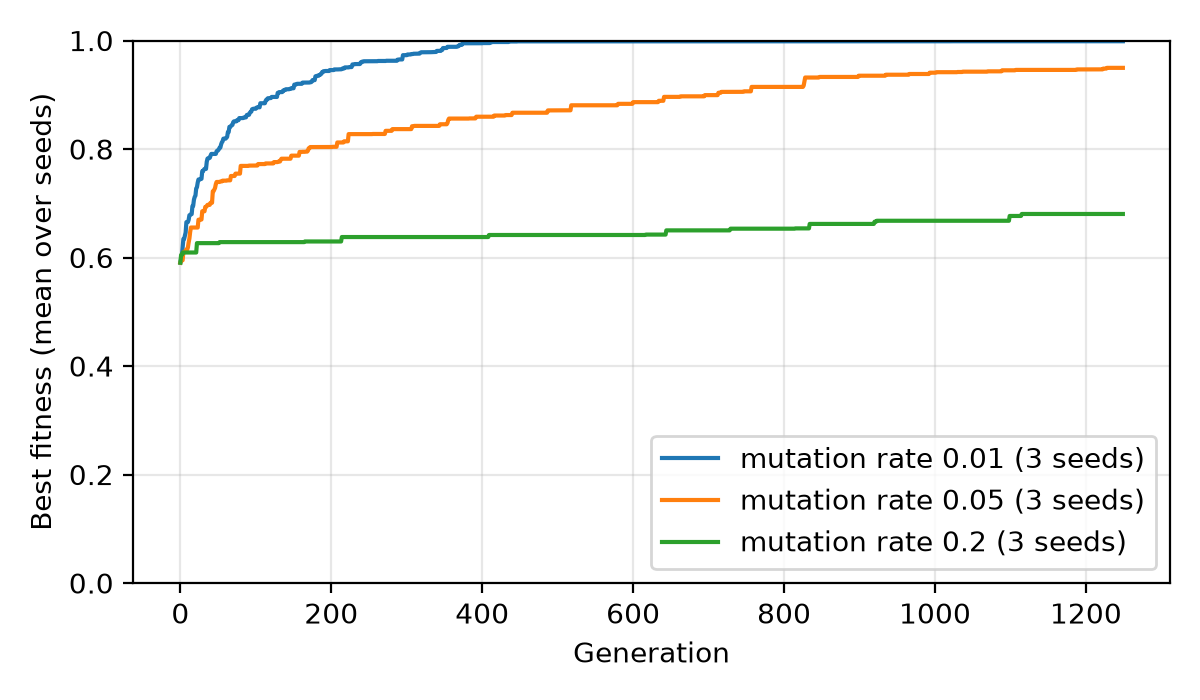
\includegraphics[width=\linewidth]{figures/comparison.png}
  \caption{Best fitness per generation for each mutation rate, averaged over 3 seeds.}
  \label{fig:comparison}
\end{figure}

\begin{table}
  \centering
  \begin{tabular}{lcccc}
    \toprule
    Rate & Seed 1 & Seed 2 & Seed 3 & Mean \\
    \midrule
    0.01 & 0.999 & 0.999 & 0.999 & 0.82 \\
    0.05 & 0.957 & 0.986 & 0.906 & 0.58 \\
    0.2  & 0.704 & 0.644 & 0.693 & 0.39 \\
    \bottomrule
  \end{tabular}
  \caption{Best fitness at the last generation (1249) per mutation rate and seed, and
    population mean fitness
    averaged over the 3 seeds.}
  \label{tab:results}
\end{table}

Figure~\ref{fig:fitness} shows the best and mean fitness of the population for one run with mutation rate 0.01, Figure~\ref{fig:comparison} compares the best fitness of the three mutation rates, and Table~\ref{tab:results} lists the final values. With the same seed, all runs start from the same initial population, with a best fitness close to 0.59.

With mutation rate 0.01, the best fitness grows quickly: it passes 0.95 between generations 186 and 340 and 0.99 by generation 374, and it ends at 0.999 on all three seeds. In the final melodies, every rule scores 1.0 except the step size, which scores 0.99. With 0.05, the GA improves more slowly and ends between 0.906 and 0.986, and only two of the three seeds pass 0.95, after generation 800. With 0.2, the best fitness stalls between 0.64 and 0.70. Its weakest rule is the chromatic approach, which ends between 0.22 and 0.39, while the breathing rule scores 1.0 for every rate and seed. In all runs, the mean fitness of the population stays well below the best one, and it drops as the mutation rate grows: 0.82 at 0.01, 0.58 at 0.05 and 0.39 at 0.2.

\subsection{Listening}
